\section{Clustering}
Clustering is a method of segmenting an image into disjoint sets known as classes. This is useful for separating types of features or objects in an image. For example in Figure \ref{fig:toycar} the toy car has been segmented from the background.

\begin{figure}[H]
	\centering
	\begin{subfigure}[b]{0.5\linewidth}
      		\centering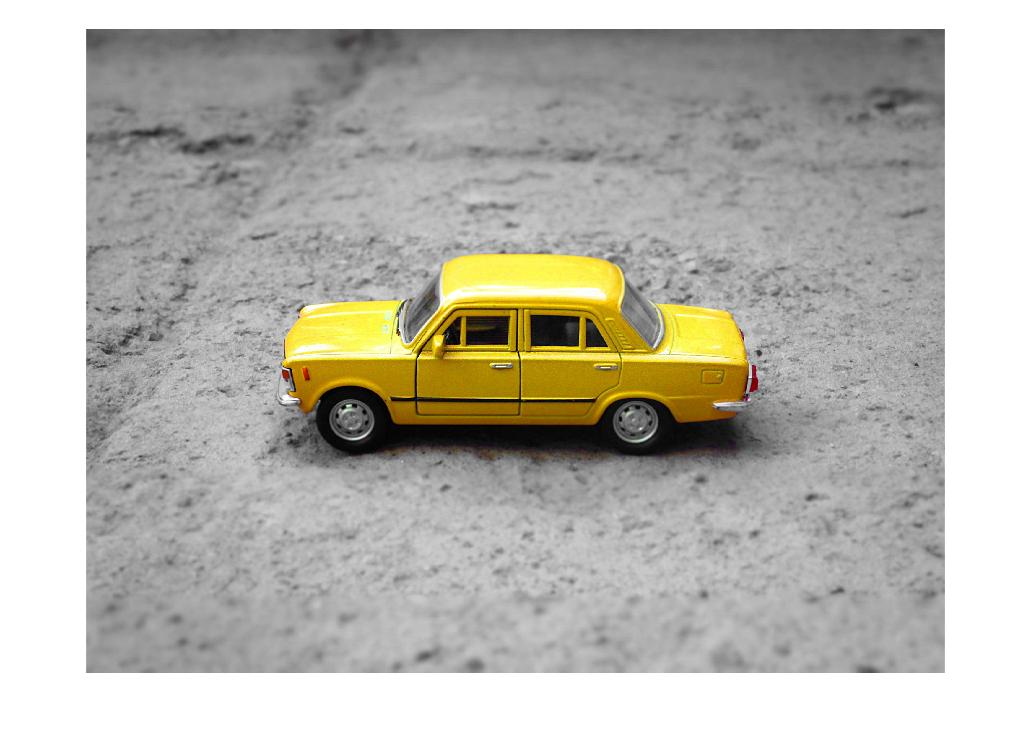
\includegraphics[width=220pt]{toyCar}
      		\caption{Image by Gustavo, Upsplash.}
		    \label{fig:toycarA}
    	\end{subfigure}%
    	\begin{subfigure}[b]{0.5\linewidth}
      		\centering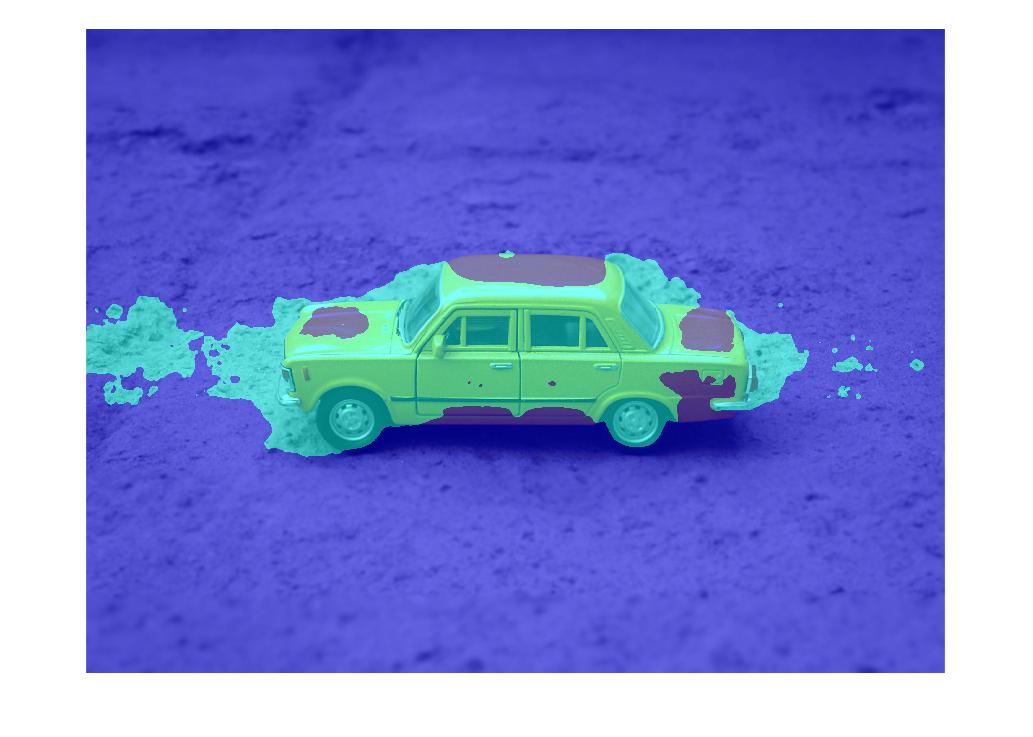
\includegraphics[width=220pt]{toycarseg}
      		\caption{Segmentation of car from background.}
       		\label{fig:toycarB}
    	\end{subfigure}
    	\caption{Segmentation of toy cars using K-Means Clustering.}
    	\label{fig:toycar}
\end{figure} 

In an image every pixel can be individually classified or groups of pixels known as superpixels may be treated as single entities. Entities are sorted based on their similarity. For example, a pixel's intensity is a feature that could be used to cluster it with other pixels of similar intensity. As seen in (\ref{eq:featurevector}) an entity's comparable traits may be represented by a feature vector. An entity may have any number of features which as also regarded as dimensions, $d$. 

\begin{equation}
    \vec{v} = 
    \begin{bmatrix}
        d_1 \\
        d_2 \\
        \vdots \\ 
        d_n
    \end{bmatrix}
    \label{eq:featurevector}
\end{equation}



\subsubsection{K-Means}
\label{subsubsection:kmeans}
K-Means is simple and reasonably fast clustering algorithm where K represents the number of cluster the algorithm should create and means refers to the average value of each cluster. Given a set of data samples their similarity is measured as the value of the Euclidean distance between them. The general form of the Euclidean distance formula is described in equation \ref{eq:euclid}, where $p$ and $q$ represent n-dimensional feature vectors. As the K-means algorithm executes, data samples are assigned to the cluster whose average value, also as a cluster centroid, is closest to the sample's own. Centroids are updated after each round of assignments until their values converge. Initially the each cluster centroid is randomly selected. The algorithm to implement the K-means method is outlined in algorithm \ref{algorithm:kmeans}.

\begin{equation}
    EuclideanDistance(p,q) = \sqrt{(p_1 - q_1)^2 + (p_2 - q_2)^2 +\hdots + (p_n - q_n)^2}
    \label{eq:euclid}
\end{equation} 

\begin{algorithm}
    \SetAlgoLined
    \KwInput{Set of data vectors X of size M} 
    \KwOutput{K sets of clustered data vectors}
    Initialize the desired number of clusters $K$\;
    Initialize a list of $K$ random cluster centroids $\mu$\;
    \While{$\mu$ elements have not converged}{
        \For{i = 0 to M}
        {
            distOld = $\inf$
            \For{j = 0 to K}{
                distnew = EuclideanDistance(X[i], $\mu[j]$)\;
                \If{distNew $<$ distOld}{
                    distOld = distNew\;
                    $\mu_j$.append(X[i])\;
                }
            }
        }
        \For{p = 0 to K}{
            centroidList.append(average($\mu[p]$))\;
        }
    }
    \caption{K Means Clustering \cite{oreilly_python}}
    \label{algorithm:kmeans}
\end{algorithm}

The best result for this method is defined as having the smallest intra-cluster variance. K-Means is disadvantaged by the implicit trait that it formulates clusters of similar sizes. This happens because the algorithm seeks to minimize variance (spread) in each cluster hence the \q{ideal} centroid placement will form distributions spherically about centroids. Figure \ref{fig:clusters} visualizes an example of clustering data where it can be observed that the cluster sizes are similar and spherical in shape. This method of clustering does not consider any probabilistic model in classifying data, this type of classification is called a \emph{hard assignment} because a data sample can belong only to one cluster. The dual of this is a \emph{soft assignment}, considers the \emph{probability} of a sample of belonging each cluster. 

\begin{figure}[H]
    \centering
    \centering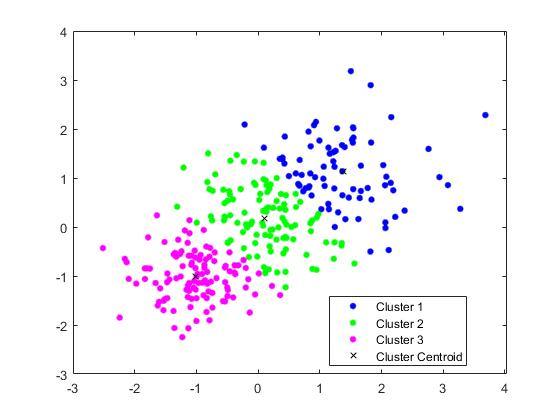
\includegraphics[width=0.9\textwidth]{kmeans_clusters}
    \caption{K-Means clustering performed on random data. \cite{matlab_clustering}}
    \label{fig:clusters}
\end{figure} 
\subsubsection{Mixtures of Gaussians}
 \label{subsection:mog}

Mixtures of Gaussians (MoG), or the Gaussian Mixture Model (GMM), is a method of clustering (see section \ref{subsection:clustering}) that is based not on distance \ref{subsubsection:kmeans} but distribution. This method of clustering was popularized by Duda and Hart in their text \emph{Pattern Classification and Scene Analysis} \cite{mog_seminal}. This method is more effective than distance based methods because it considers the covariance of the data. Note that for K-Means clustering the distributions were spherical, but if the true clusters were more elliptical then K-Means would fail to cluster them properly. Figure \ref{fig:cluster_shapes} compares what these cluster shapes might look like and the arrows indicate the location, the arrows indicate data points that are ambiguous.

\begin{figure}[h]
	\centering
	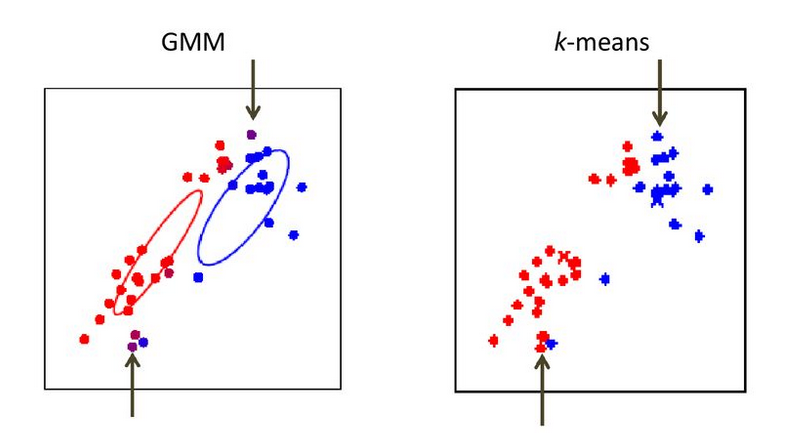
\includegraphics[width = 0.9\textwidth]{litreview/computervision/mog/mog_vs_kmeans.png}
	\captionsetup{format = hang}
	\caption{Comparison of K-Means cluster shape to GMM cluster shape. Img: Hongning Wang, University of Virginia }
	\label{fig:cluster_shapes}
\end{figure}
	
The basis of the Gaussian Mixture Model is of course the Gaussian Distribution function \ref{section:gaussian}. It is useful for probabilistic clustering because, as the Central Limit Theorem States, the distribution of the average value of the subsets of any data set will approximately converge to a Normal distribution as the number of terms in the subsets increases \cite{patterns_machine_learning}. The Mixture of Gaussian for the random variable $\boldsymbol{x}$ is achieved by super-positioning the distributions of random variable for each cluster. Equation \ref{eq:mog} describes the super-positioning of $K$ distributions for random variable $\boldsymbol{x}$, the resulting curve models the distribution of the random variable. 

\begin{equation}
p(\boldsymbol{x}) = \sum^{K}_{k = 1}\pi_k \mathcal{N}(\boldsymbol{x}|\boldsymbol{\mu_k}, \boldsymbol{\Sigma_k})
\label{eq:mog}
\end{equation}

The variable $\pi_k$ is known as the \emph{mixing coefficient} of a Gaussian distribution which controls the weighting of a particular distribution in the mixture. The sum of the mixing ratios is 1 because the complete mixture distribution represent the probability of a sample belonging to any one cluster and it must belong to one, hence

\[\sum_{k=1}^K\pi_k = 1\]

To help to understand how equation \ref{eq:mog} came about consider the random variable $\boldsymbol{z}$ of dimension K which is a binary random variable, meaning it can only have value 1 or 0. Only one element of $\boldsymbol{z}$ can be equal to 1 and all others must be 0, thus

\[\sum_{k=1}^Kz_k = 1\]

Hence there are K possible combinations of the vector $\boldsymbol{z}$. The marginal distribution over $\boldsymbol{z}$ is defined in terms of the mixing coefficients, 

\[p(z_k = 1) = \pi_k\]

That is to say the probability of $z_k$ = 1 is equal to the mixing coefficient of Gaussian distribution k. This can also be written

\[p(\boldsymbol{z}) = \prod^K_{k=1}\pi^{z_k}_k\]

The significance of $\boldsymbol{z}$ represents the assignment of a sample to a cluster which is why only one of its elements can be 1. To observe the Gaussian distribution of $\boldsymbol{z}$ in cluster $K$ we set $z_k = 1$ as described by the condition distribution,

\[p(\bm{x}|\boldsymbol{z}) = \mathcal{N}(\boldsymbol{x}|\boldsymbol{\mu_k}, \boldsymbol{\Sigma_k}) \]

Finally we can determine that the marginal distribution of $\boldsymbol{z}$ which is described by \ref{eq:mog} using the marginal distribution $p(\boldsymbol{z})$ and the conditional distribution $p(\bm{x}|\bm{z})$ as 

\begin{align}
	p(\bm{x}) 	&= p(\bm{z})p(\bm{x}|\bm{z})
				&= \sum^{K}_{k = 1}\pi_k \mathcal{N}(\boldsymbol{x}|\boldsymbol{\mu_k}, \boldsymbol{\Sigma_k})
\label{eq:mog_derive}
\end{align}

Figure \ref{fig:mog_compare}

\begin{figure}[htbp]
    \centering
     \begin{subfigure}[b]{0.45\textwidth}
        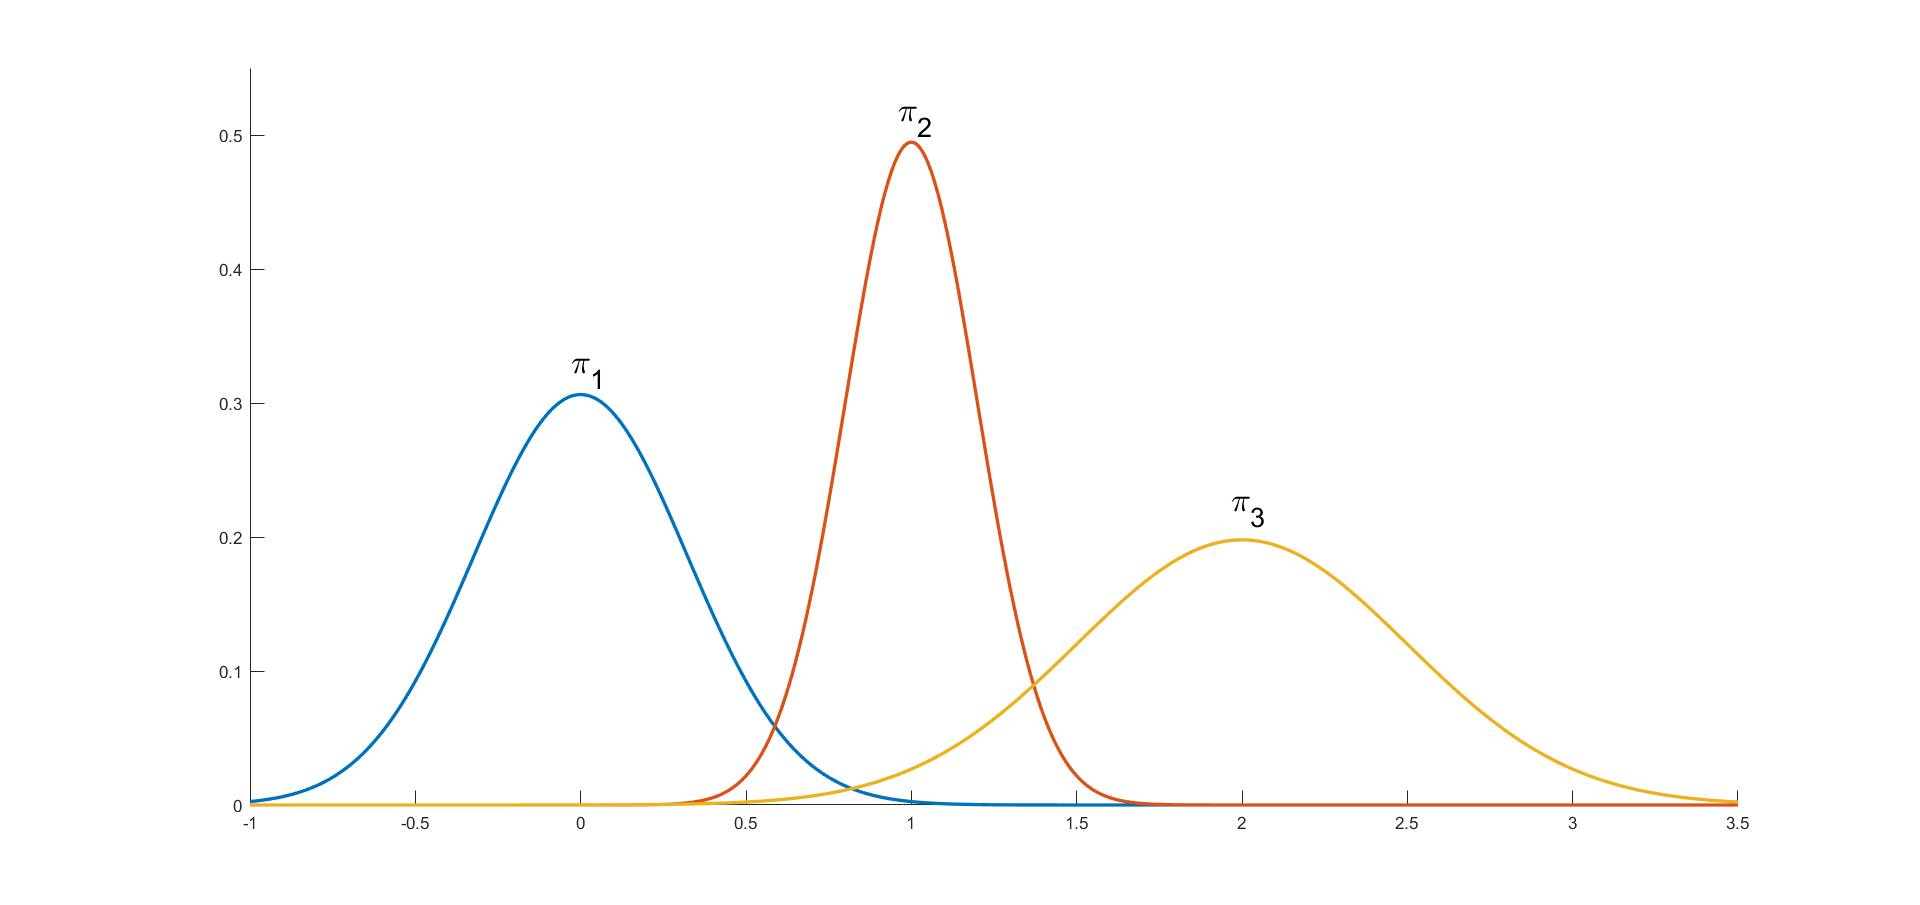
\includegraphics[width=\textwidth]{litreview/machinelearning/clustering/mog/individual_gauss.png}
	\captionsetup{format = hang}
        \caption{Three individual cluster distributions.}
        \label{fig:mog_singles}
    \end{subfigure} 
    \begin{subfigure}[b]{0.45\textwidth}
        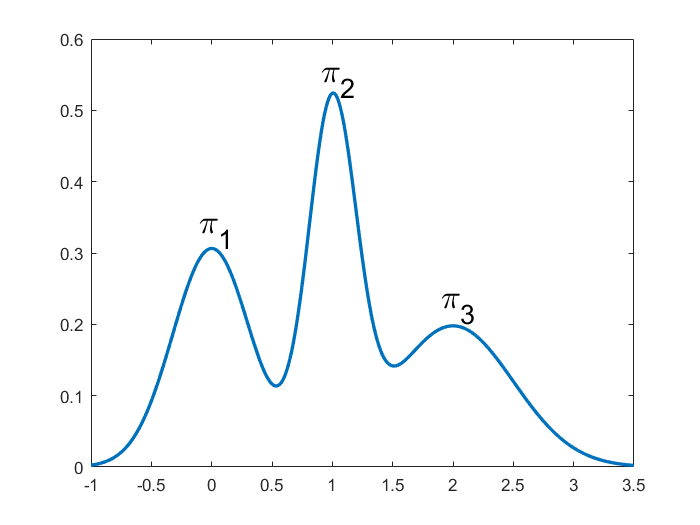
\includegraphics[width=\textwidth]{litreview/machinelearning/clustering/mog/combined_mog.png}	
	\captionsetup{format = hang}
        \caption{Super-positioned Gaussian distributions}
        \label{fig:mog_combined}
    \end{subfigure}
    \captionsetup{format = hang}
    \caption{Visualization of a Mixture of Gaussians for 1D dataset.}
    \label{fig:mog_compare}
\end{figure}











Initially, K Gaussian functions are randomly generated corresponding to K clusters. If a dataset has low dimensionality, by taking a histogram of its values the Gaussians' initial conditions can be approximated, as in Figure \ref{fig:histGauss}. By super-positioning all of the Gaussians a sample's complete probabilistic model is created, i.e. a model for \emph{all} clusters, see Figure \ref{fig:histCurve}. 

\begin{figure}[H]
	\centering
	\begin{subfigure}[b]{0.5\linewidth}
            \centering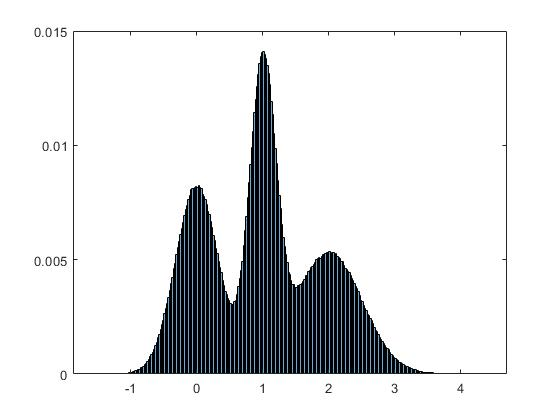
\includegraphics[width=215pt]{histGauss}
      		\caption{Normalized Histogram of 1D samples.}
		\label{fig:histGauss}
    	\end{subfigure}%
    	\begin{subfigure}[b]{0.5\linewidth}
      		\centering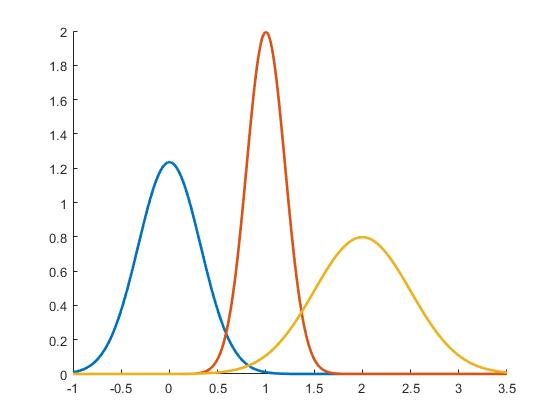
\includegraphics[width=215pt]{hist_gauss_curve}
      		\caption{Gaussians derived from 1D histogram.}
       		\label{fig:histCurve}
		\end{subfigure}
		\caption{Formulation of Mixture of Gaussians.}
    	\label{fig:mixture}
\end{figure}

With each iteration of the GMM algorithm the parameters of the model's component Gaussians are tuned according to the covariance between samples in each cluster. In \ref{eq:cov} $X$ and $Y$ are the variables being compared, $\overline X$ and $\overline Y$ are variable means and $n$ is the number of samples. For a multidimensional dataset a covariance matrix $\bm{\Sigma_k}$ will be generated and each Gaussian will require a mean vector $\bm{\mu_k}$ as opposed to a scalar. 

\begin{equation}
Cov(X, Y) = \frac{\Sigma(X_i-\overline X)(Y_j-\overline Y)}{n}
\label{eq:cov}
\end{equation}



The algorithm seeks the highest covariance possible in each of its clusters. It is by considering the covariance of samples that the GMM is able to best classify ambiguous samples. The higher the covariance (aka correlation) between sample dimensions the more likely it is they belong in the same cluster. This can observed in Figure \ref{fig:mogcov}, the data being clustered is the same as in Figure \ref{fig:clusters} but notice the elliptical shape of the Gaussian cluster distributions as opposed to the spherical shape of K-Means clustering.

\begin{figure}[H]
	\centering
	\centering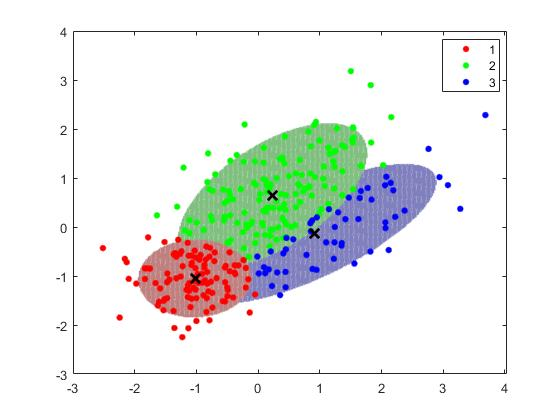
\includegraphics[width=450pt]{mog}
	\caption{Clustering using GMM. X marks cluster mean.}
	\label{fig:mogcov}
\end{figure}
  
In Figure \ref{fig:histScale} the Gaussians from Figure \ref{fig:histCurve} have been scaled to have the amplitudes $\pi_1 = 0.3$, $\pi_1 = 0.5$ and $\pi_1 = 0.2$. These are weightings that give the mixing ratio of the GMM and represent each cluster's proportion of the total samples. The more samples a cluster contains the more likely it is a sample belongs to it. The sum of ratios must add to one because the probability a sample belongs to at least one cluster is one, as defined in \ref{eq:gauss_weight1} and \ref{eq:gauss_weight2}.

\begin{equation}
    0\leq \pi_k \leq 1
\label{eq:gauss_weight1}
\end{equation}
\begin{equation}
    \sum_{k=1}^{K}\pi_k = 1
\label{eq:gauss_weight2}
\end{equation}


\begin{figure}[H]
    \centering
    \centering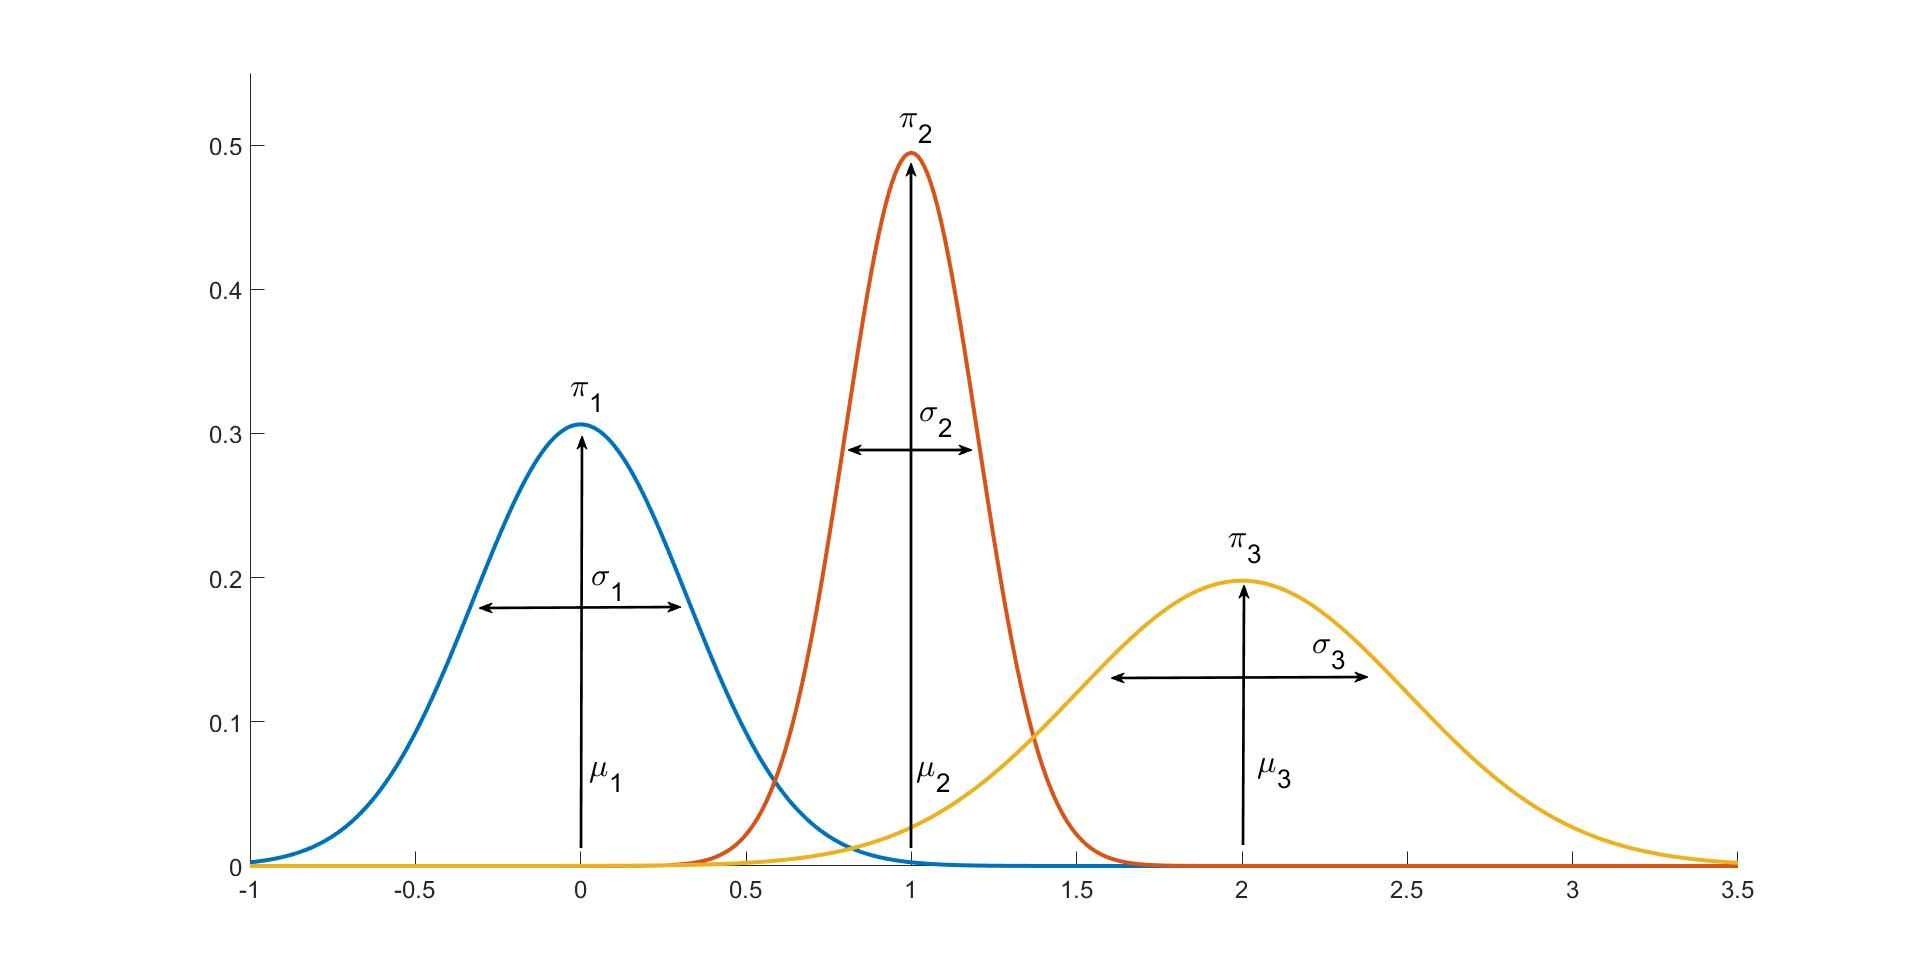
\includegraphics[width=450pt]{gauss_mix_scale}
    \caption{Individual Gaussians with scaled weightings.}
    \label{fig:histScale}
  \end{figure} 

Each Gaussian's three parameters, mean $\bm{\mu}_k$, ampltidue $\pi_k$ and covariance $\bm{\Sigma}_k$ are updated following each iteration of the algorithm according to the 'Expectation Maximization' algorithm.

\subsubsection{Expectation Maximization}

Expectation Maximization (EM) is a method of updating the parameters of cluster Gaussians that seeks to maximize a sample's likelihood of belonging to said Gaussians (\ref{eq:likelihood}). 

\begin{equation}
\label{eq:likelihood}
p(x) = \sum^K_{k=1} \pi_k \mathcal{N}(x|\bm{\mu}_k, \bm{\Sigma}_k)
\end{equation}

A binary indicator $z_{i}$ exists for every sample $x_i$, it is 1 if the sample belongs in the cluster $k$ and 0 otherwise such that $z_{ik} \in \{0, 1\}$ and $\sum_k z_{ik} = 1$. If the data is multidimensional then the sample and inidicator are both vectors, $\bm{x}$ and $\bm{z}$. The marginal probability $p(\bm{z}_{k} = 1)$ is the probability that a sample $\bm{x}$ is in cluster $k$. This quantity is completely specified by the mixture weight $\pi_k$ for each Gaussian because the area under a Gaussian component is equal to its mixing ratio, i.e.

\begin{equation}
	\label{eq:marginalk}
	p(\bm{z}_{k}=1) = \pi_k 
\end{equation}
	
If we know that a sample $\bm{x}$ is from cluster $k$ the \emph{likelihood} of seeing it in the associated Gaussian is the value of the Gaussian at that point,
\begin{equation}
	\label{eq:cond}
	p(\bm{x}\, |\, \bm{z}_{k} = 1) = \mathcal{N}(\bm{x}\, |\,\bm{\mu_k}, \bm{\Sigma_k})
\end{equation}

The conditional probability of $\bm{z}_{ik}$ given the value of sample, $\bm{x}_i$ is denoted as $\gamma(\bm{z}_{ik})$. This is the probability that a sample belongs to cluster $k$ given its value $\bm{x}_i$ and is the quantity of interest when trying to classify a sample.  Using Bayes Theorem [REF APPENDIX] quantity can be found 

\begin{align}
	\gamma(\bm{z}_{ik}) \equiv p(\bm{z}_{ik} =1 | \bm{x}_i)
	\label{eq:gamma2}
	&= \frac{p(\bm{z}_{ik}=1)p(\bm{x}_i\, |\, \bm{z}_{ik} = 1)}{\sum^K_{j=1}p(\bm{z}_{jk}=1)p(\bm{x}_j\, |\, \bm{z}_{jk} = 1)}\\ 
	\label{eq:gamma3}
	&= \frac{\pi_k\, \mathcal{N}(\bm{x}\,|\,\bm{\mu_k},\bm{\Sigma_k})}{\sum_{j=1}^{K}\pi_k\, \mathcal{N}(\bm{x}\,|\,\bm{\mu_k},\bm{\Sigma_k})}
\end{align}


To maximize the likelihood of each sample being in each Gaussian the distribution parameters are modified. This is achieved by taking derivatives of the log of the likelihood function (\ref{eq:likelihood}) with respect to each Gaussian parameter and setting the result to 0 to find local maxima. To take the log of the likelihood function assume all samples in are in an $N \times D$ matrix $\bm{X}$ and the corresponding indicators are in an $ N \times K$ matrix $\bm{Z}$. 

\begin{equation}
\label{eq:log}
ln\,p(X|\bm{\pi}, \bm{\mu}, \bm{\Sigma}) = \sum_{n=1}^N
ln \Bigg\{ \sum_{k=1}^K \pi_k\mathcal(N)(\bm{x}_n|\bm{\mu}_k,\bm{\Sigma}_k)\Bigg\}
\end{equation}







\centerline{}

The EM algorithm is comprised of [X] steps

%% EM STEPS %%
\begin{enumerate}
	\item Generate the initial K Gaussian parameters mean $\bm{\mu}_{k}$, covariance $\bm{\Sigma}_k$ and mixing ratios $\pi_k$ either randomly or informed by a histogram.
	\item Estimate the likelihood sample n was generated by cluster k for all samples. 
	\begin{equation}
		\gamma(\bm{z}_{ik})=\frac{\pi_k\, \mathcal{N}(\bm{x}\,|\,\bm{\mu_k},\bm{\Sigma_k})}{\sum_{j=1}^{K}\pi_k\, \mathcal{N}(\bm{x}\,|\,\bm{\mu_k},\bm{\Sigma_k})}
	\end{equation}

	\item Maximize the Gaussian parameter using derivatives of log likelihood for each parameter.
	\begin{align}	
	\label{eq:mean}
	\bm{\mu}_{k}^{new} &= \frac{1}{N_k}\sum_{n=1}^N \gamma(z_{nk} ) \bm{x}_n \\
	\label{eq:covariance}
	\bm{\Sigma}_k^{new} &=  \frac{1}{N_k}\sum_{n=1}^N\gamma(z_{nk})(\bm{x}_n- \bm{\mu}_k^{new})(\bm{x}_n - \bm{\mu}_k^{new})^T \\
	\label{eq:ratio}
	\pi_k &= \frac{N_k}{N}
	\end{align}
	where \newline
	\[N_k = \sum_{i} z_{ik}\]
	\item Repeat steps 2 and 3 until convergence of log likelihood (\ref{eq:likelihood}) or parameters. 
\end{enumerate}

The Gaussian Mixture Model method of clustering is computationally complex compared to K-Means however it's ability to differentiate ambiguous samples by considering covariance is superior. 


